\subsection{Postopek izdelave}
Za izdelavo sta nujna dva vpetja. Potrebovali bomo 2 noža in 2
svedra. En nož je profilni nož, zbrušen v konico pod kotom 45°, eden pa
bo odrezni nož s ploščico iz karbidne trdnine, širine 1,5 mm.
Centrirni sveder je brušen po meri z zaokrožitvijo, vijačni
sveder pa bo standardni HSS-sveder premera ø1,4 mm. Spodaj v Tabeli \ref{tabela_operacij}
so prikazane vse operacije s podatki vrtljajev in željenega pomika.

\begin{table}[H]
	\caption{Tabela operacij}
	\label{tabela_operacij}
	\begin{center}
		\begin{tabular}{|c|c|c|c|c|}
			\hline
			Št. & Operacija      & Naziv orodja              & Vrtljaji [\( \frac{vrt}{min}\)] & Željen pomik [\( \frac{mm}{vrt}\)] \\
			\hline
			1   & Struženje roba & Profilni nož 8 x 8        & 2000                            & 0,04                               \\
			\hline
			2   & Središčenje    & Profilni sveder $\phi$ 6  & 4000                            & 0,04                               \\
			\hline
			3   & Vrtanje        & Vijačni sveder $\phi$ 1,4 & 4000                            & 0,03                               \\
			\hline
			4   & Odrez          & Odrezni nož               & 2000                            & 0,02                               \\
			\hline
			5   & Povrtavanje    & Profilni sveder $\phi$ 6  & 2000                            & 0,03                               \\
			\hline
		\end{tabular}
	\end{center}

\end{table}

Spodaj na Sliki \ref{skica_orodij} so prikazane skice orodij.  Od leve proti desni: profilni nož 8 x 8,
odrezni nož, profilni centrirni sveder, vijačni sveder.

\begin{figure}[H]
	\begin{center}
		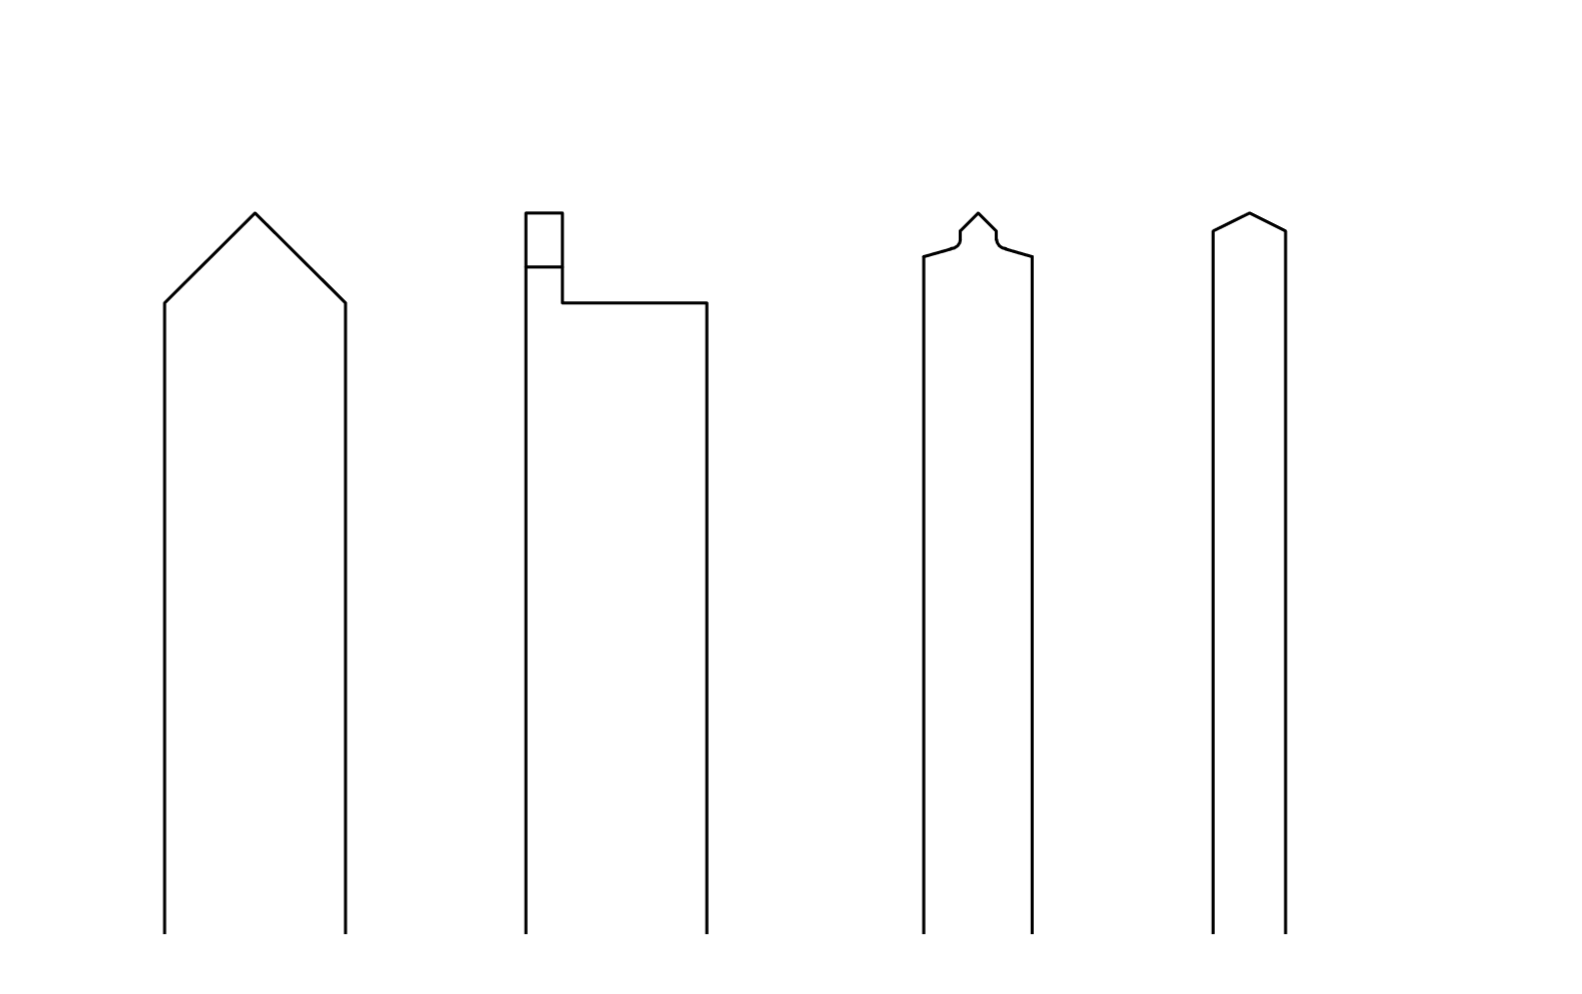
\includegraphics[width=8cm]{skica_orodij.png}
		\caption{Skica orodij
			\cite{lasten}}
		\label{skica_orodij}
	\end{center}
\end{figure}

Te parametre sem približno izbral glede na izkušnje. Ker stroj nima
menjalnika za hitrost glavnega vretena, sem izbral enotno hitrost
2000 \( \frac{vrt}{min} \). Za svedre sem pa uporabil posebnost tega stroja,
da lahko svedre posebej vrti v nasprotno smer od glavnega vretena, kar pomeni,
da se hitrosti vrtenja seštevajo in tako lahko dosežemo veliko večje hitrosti
z manjšo obrabo stroja. To pomeni, da se morajo svedri vrteti s hitrostjo
2000 \( \frac{vrt}{min} \). Za povrtavanje luknje z druge strani pa stroj
kos preprime s posebnim držalom, ki se ne mora vrteti, zato sem uporabil največjo
hitrost gnanega orodja; 2000 \( \frac{vrt}{min} \).

Ker nam stroj na krivulje omogoča več obdelav naenkrat, sem prekril
struženje roba skupaj s središčejem in odrez z vrtanjem luknje.
Ker se povrtavanje luknje z druge strani izvaja neodvisno od
glavnega vretena, lahko čas te operacije ignoriramo pri času
celotnega cikla.
S tem lahko čas cikla zmanjšamo na približno 10 s.
